\documentclass[11pt]{article}
\usepackage{geometry}                % See geometry.pdf to learn the layout options. There are lots.
\usepackage{url}
\geometry{letterpaper}                   % ... or a4paper or a5paper or ...
%\geometry{landscape}                % Activate for for rotated page geometry
%\usepackage[parfill]{parskip}    % Activate to begin paragraphs with an empty line rather than an indent
\usepackage{graphicx}
\usepackage{amssymb}
\usepackage{epstopdf}
\usepackage{authblk}
\usepackage{color}
\newcommand{\hilightr}[1]{\color{red}{#1}}
\newcommand{\hilightg}[1]{\color{green}{#1}}
\newcommand{\hilightb}[1]{\color{blue}{#1}}

%\usepackage{algorithm}
%\usepackage{algorithmic}
\usepackage[ruled, noend, noline, algo2e]{algorithm2e}


\DeclareGraphicsRule{.tif}{png}{.png}{`convert #1 `dirname #1`/`basename #1 .tif`.png}

\begin{document}


\title{KHYRank: Using Retweets and Mentions to Predict Influential Users}


\author[1]{Aron Yu}
\author[1]{C. Vic Hu}
\author[2]{Ann Kilzer}
\affil[1]{Dept.\,of Electrical Engineering, The University of Texas at Austin}
\affil[ ]{{\small\tt\{aron.yu, cvhu\}@utexas.edu}}
\affil[2]{Dept.\,of Computer Science, The University of Texas at Austin}
\affil[ ]{{\small\tt\{akilzer\}@cs.utexas.edu}}

\maketitle

\date{}                                           % Activate to display a given date or no date


\maketitle

\begin{abstract}
Determining influential users is a widely studied problem in online social networks.  In this study, we use real data from Twitter: the social graph and a set of tweets from a five month period.  Specifically, we examine retweets and mentions, which indicate a response or citation.  We argue that these are better indicators of influence than mere follower count or PageRank.
	We present KHYRank, an algorithm for  determining influence based on the graph structure, and probability of a user mentioning or retweeting another user.  Not only does our algorithm successfully find celebrities and content sources, but it also can be efficiently run on a desktop using MATLAB.
\end{abstract}


\section{Introduction}

We've all heard about viral marketing.  Even Forbes.com compared the social graph to ``crude oil," describing it as an ``unrefined and complex natural resource containing many riches" \cite{forbes}.   Maciej Ceglowski, the developer behind Pinboard.in quipped ``Social networks exist to sell you crap. The icky feeling you get when your friend starts to talk to you about Amway, or when you spot someone passing out business cards at a birthday party, is the entire driving force behind a site like Facebook" \cite{maciej}.

Advertisers want to run the most effective campaign using a limited budget. The whole idea behind viral marketing is to target users who will spread the word to their friends.
But how do we choose which users to target?  Our project is to find a scalable method for finding the most influential users in a social graph.  We hypothesize that we can measure an individual's influence by the number of \emph{repeaters} they connect to.  By repeaters, we mean those users who redistribute content (Think Twitter's ``retweets," Google+ and Facebook's ``Share" features).

%TODO: neaten up

\section{Background}

\subsection{Twitter}
Twitter is an online social network that specializes in ``microblogging,'' sharing text snippets, or ``tweets,''  of no more than 140 characters.  It is a directed graph: you may follow others, subscribing to their tweets, but they may not necessarily follow you.  Features of the service include the ability to ``retweet,'' or repeat, verbatim, another user's post.  Additionally, users label their tweets via hashtags, short strings beginning with \#, which provide some context to the tweet.  For instance, a current popular hashtag is ``\#OcuppyOakland,'' which quickly provides context to tweets about the current political protests.  Another feature is to directly reference users by putting an @ before their screen name.  We will refer to this as an ``@ mention, (at mention).

Twitter distinguishes itself from other popular social networks in that it is easy to repeat content, either via retweets or repeating a hashtag.  Posts are by default public, and twitter is a popular platform for celebrities, brands, and organizations to connect with their followers.  Typically, users read tweets in a stream format containing live updates from all the users they follow.

Our study focuses on retweets and mentions.  We argue that these metrics are useful in finding influence, as they demonstrate a user responding to a specific piece of information from a source.  In the retweet case, the user is just mirroring the source's information to his or her followers.  Note that retweets may propagate along a chain of users.  For instance, consider when user $A$ is followed by user $B$, who is followed by user $C$.  If $B$ retweets $A$'s tweet, then the tweet shows up in $C$'s stream with both the source's name ($A$) and the last link in the chain ($B$).  In the @ mention case, the user is typically addressing some topic from a source, or calling them out by name.




%TODO: expand

\subsection{Data}

We obtained our data from multiple sources:.  The first dataset is a set of tweets collected between September 2009 and January 2010 \cite{chengCIKM2010}.  The data set contains 113,515 Twitter users and 3,844,612 updates from the users. The original test and training set were not well balanced, and contained few overlapping users. We redivided the users by time, so we could use training data from an earlier time period to predict influence in a later time period.  The new training set contains data from September through November, 2009, while the new test set contains data from December 2009 and January 2010.

The second dataset is a crawl of the entire Twitter graph from June 2009 \cite{Kwak10www}.  According to the authors, it is a crawl of the entireTwitter site with 41.7 million user profiles and 1.47 billion edges.

The authors of the twitter graph also provided a mapping from Twitter usernames to user ids.  Lastly, we also used the info chimps API to obtain mapping information \cite{infochimpsAPI}.  This was helpful when we parsed usernames from @ mentions and retweets, because most of the data is stored according to user id.


\subsection{Implementation}

We implemented our code in python and MATLAB.  Python was used for constructing an adjacency matrix, and parsing the tweet dataset.  We combed our tweet data for the retweets and @ mentions.  
Once we had our data in a suitable format, we used MATLAB for the heavy lifting.

\section{Methodology}

We devise a new algorithm to determine influence using retweet and @ mention data. More specifically, we are looking at the number of times a user has been retweeted or been mentioned by his or her followers. The first step is to construct the influence matrix which contains the probability of one user influencing another user for all users in the dataset. The next step is to calculate the influence ' using the influence matrix using different methods. The last step is to simulate the propagation of information in the user network to come up with the simulated influence '. We compare our algorithm's results with traditional influence metrics such as PageRank and degree count.

We define a retweet to be a tweet leading with ``RT @user'' and an @ mention to be a tweet containing ``@user'' anywhere besides the beginning of the tweet. Both retweets and @ mentions are subsets of the overall number of tweets by the user. 

\subsection{Influence Matrix Calculation Algorithm}

Using the adjacency matrix \textbf{A}, we create two matrices from the training data set.  The retweet matrix \textbf{R} counts the number of times a user in row $i$ retweets about a user in column $j$.  The mention matrix \textbf{M} counts the number of times a user in row $i$ mentions about a user in column $j$.  The sum of each row represents the total number of times each user retweeted or mentioned about another user. We use these statistics to compute the Influence matrix \textbf{IF}, which contains probability of a user in row $i$ influencing a user in column $j$.  See algorithm \ref{alg:imc} for details.

\begin{algorithm2e}[h]
%\dontprintsemicolon
\caption{Influence Matrix Calculation}
\label{alg:imc}

\KwIn{Adjacency matrix \textbf{A}, Retweet matrix \textbf{R}, Mention matrix \textbf{M}}

\KwOut{Influence matrix \textbf{IF}}

\smallskip

\ForEach {user $u_i$}{
	\ForEach {user $u_j \neq u_i$}{
	$P(u_j$ rt $u_i) = \frac{\textrm{\# of times  $u_j$  retweeted $u_i$}}{\textrm{total \# of retweets by $u_j$}}$\; \label{eq1}
	\smallskip
	$P(u_j$ m $u_i) = \frac{\textrm{\# of times  $u_j$  mentioned $u_i$}}{\textrm{total \# of mentions by $u_j$}}$\; \label{eq2}
	\smallskip
	$w_{rt}(j) = \frac{\textrm{total \# of retweets by $u_j$}}{\textrm{total \# of retweets and mentions by $u_j$}}$\; \label{eq3}
	\smallskip
	$w_{m}(j) = \frac{\textrm{total \# of mentions by $u_j$}}{\textrm{total \# of retweets and mentions by $u_j$}}$\; \label{eq4}
	\smallskip
	
	
	$\textbf{IF}_{i,j} = P(\textrm{$u_i$ influences $u_j$} )= w_{rt}(j)P(u_j$ rt $u_i) + w_m(j)P(u_j$ m $u_i)$\; \label{eq5}

	}
}
\end{algorithm2e}

We define the probability of user $i$ influencing user $j$ $P(u_j$ influences $u_i)$ to be the weighted sum of the the probability of user $j$ retweeting about user $i$ $P(u_j$ rt $u_i)$ and the probability of user $j$ mentioning about user $i$ $P(u_j$ m $u_i)$. We define the weights $w_{rt}(j)$ and  $w_{m}(j)$ proportionally to the total number of retweets and mentions by each user. We see here that if user $j$ tends to retweet about $i$ out of all his retweets, then it is more likely that user $j$ will retweet about user $i$ if user $j$ does decide to retweet about someone. It also follows logically that if user $j$ tends to retweet more than @ mention when passing down a piece of information, more weight should be given to the retweets of user $j$. 

It is important to note that user $i$ can only influence user $j$ if user $j$ is a follower of user $i$. In order for user $i$ to have a higher probability of influencing user $j$, user $j$ must be willing to not just pass down information but to pass down user $i$'s information specifically. Figure \ref{connectionPlot} represents a spy plot of the adjacency matrix \textbf{A} and the computed influence matrix \textbf{IF} using the first 15,000 users in our dataset. We see that though the users are tightly connected by following one another, the actual influence among the users is rather sparse. Therefore, the influence matrix proves to be a more accurate representation of the influence among the users.

\begin{figure}[htbp]
\begin{center}
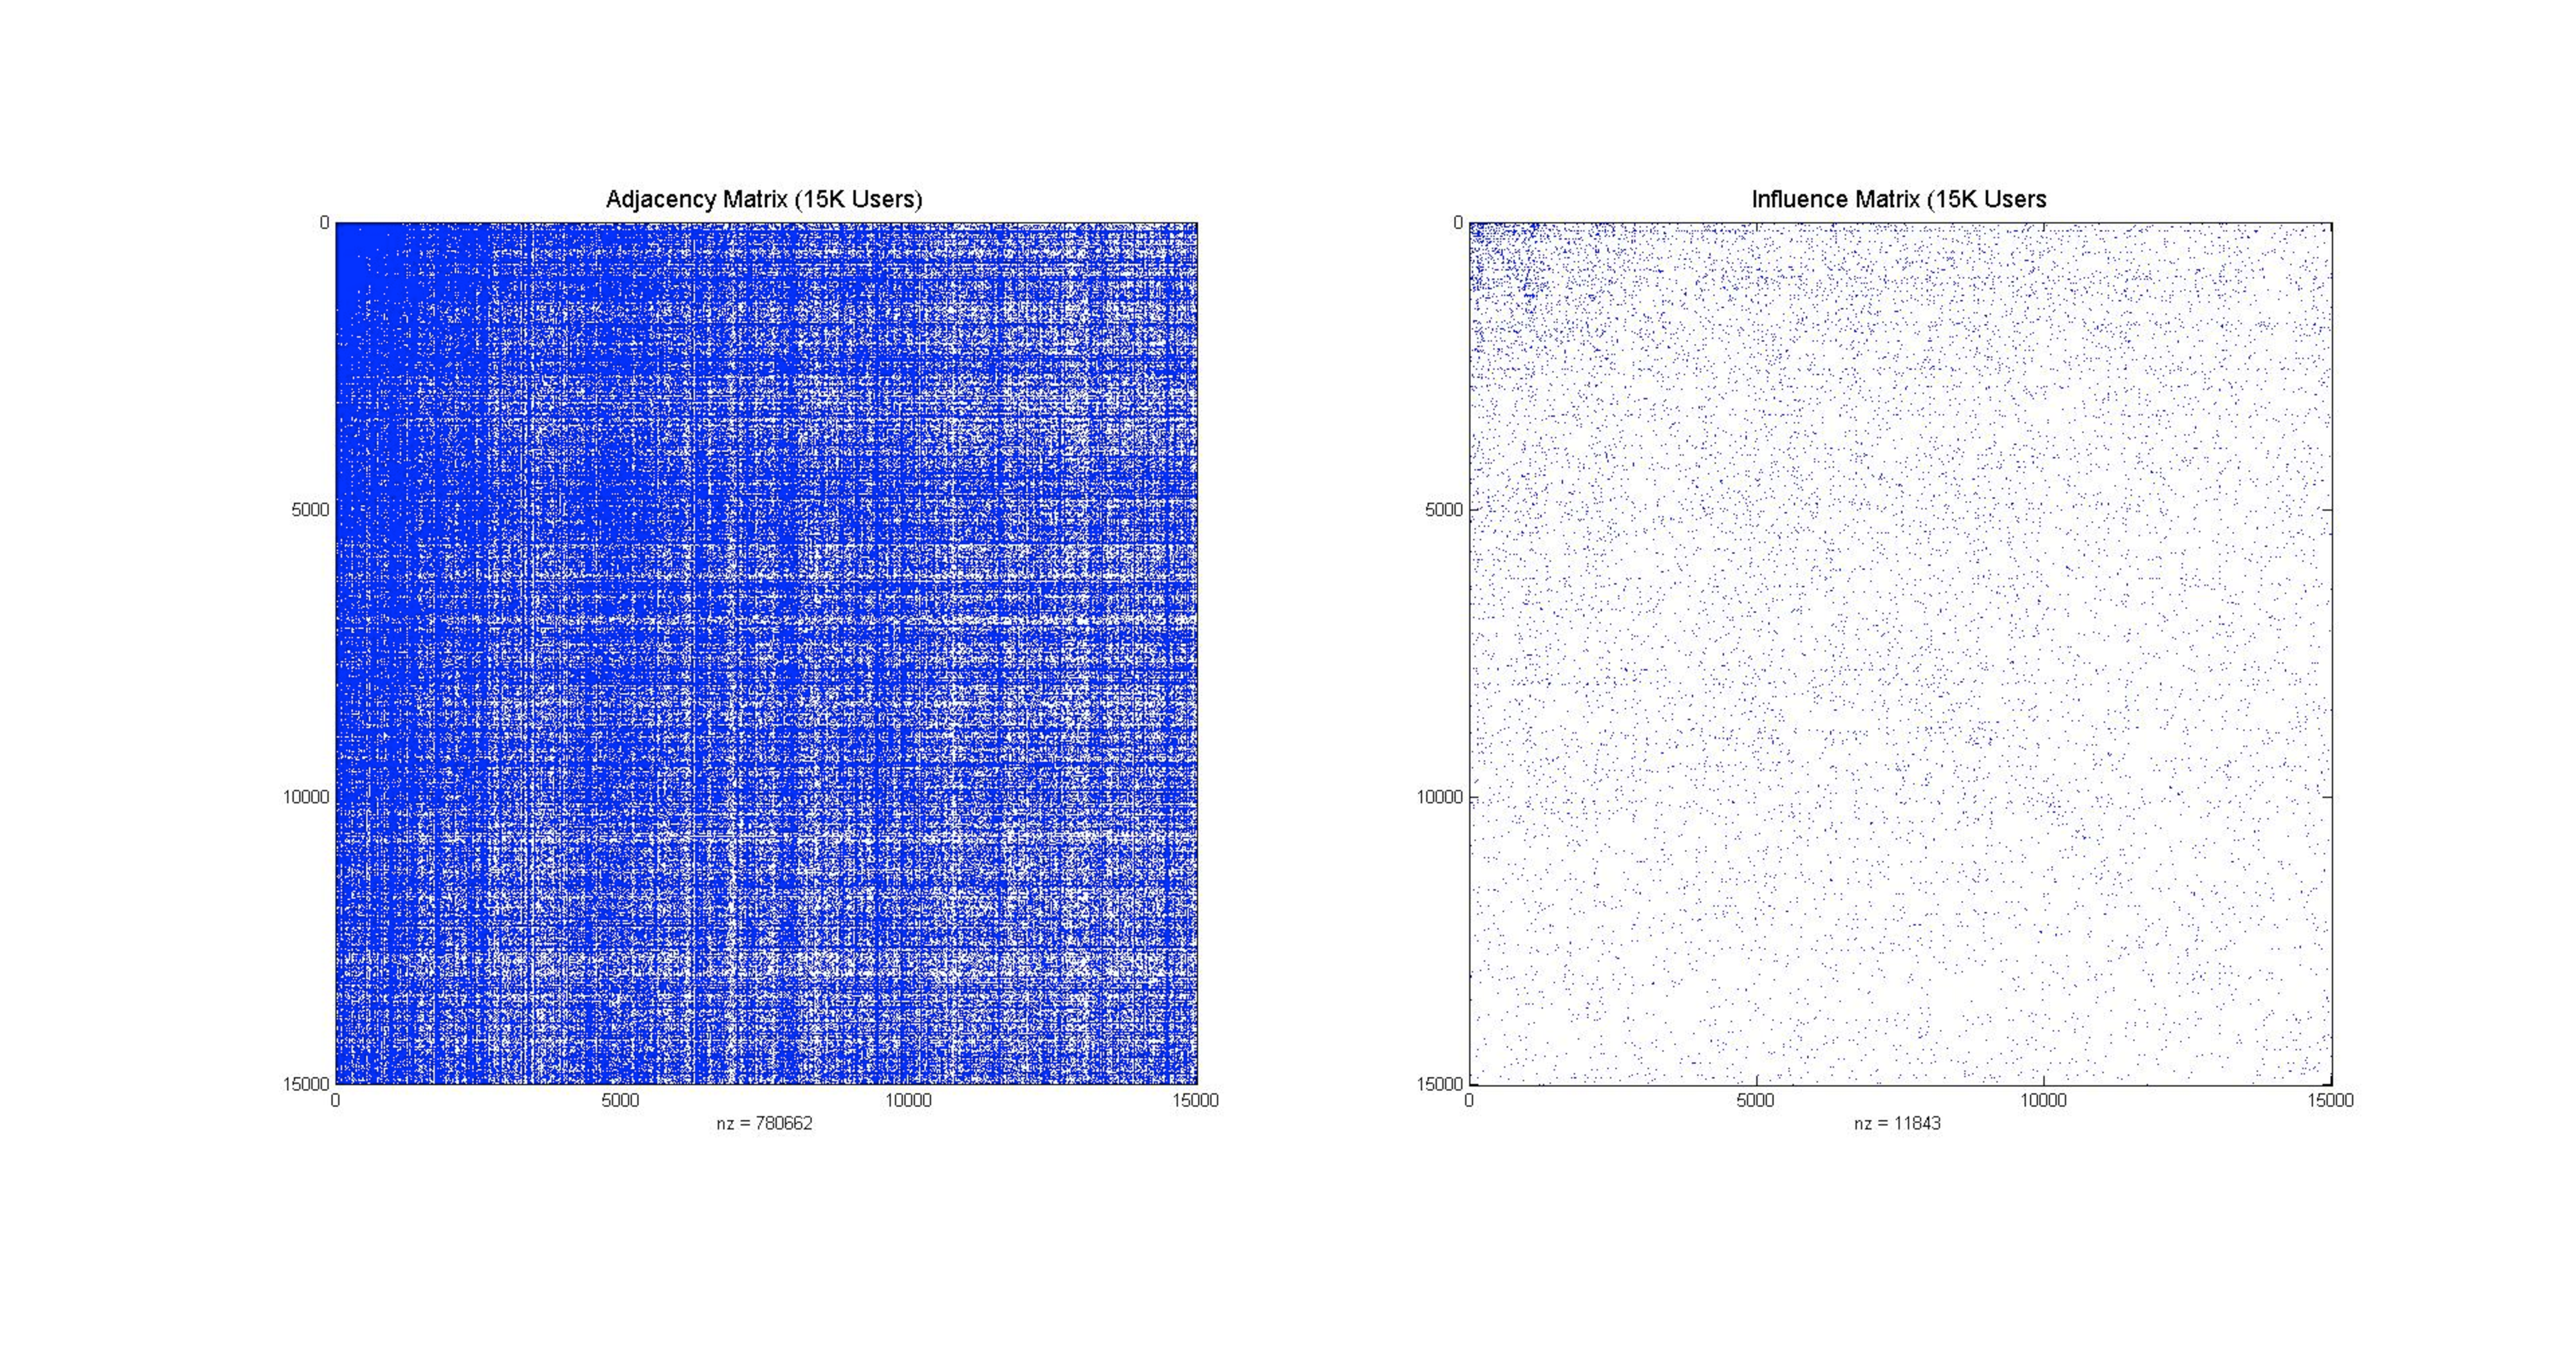
\includegraphics[width=6.5in]{connection_plot_15K}
\label{connectionPlot}
\caption{Connection Graph for 15,000 Users}
\end{center}
\end{figure}


\subsection{Influence ' Calculation}

Using the influence matrix, we now compute the influence ' and rank the users according to their influence level. We implement 3 different computation methods with minor modifications between the methods. The following equations represent the influence ' computation for a single user $u_s$. $T_s$ is the total number of tweets by user $u_s$.

\-\\

\noindent\textbf{2-Layer Score:} Looking at the immediate followers of $u_s$ and summing up the probability of $u_s$ influencing each of the followers. We mutiply the result by $T_s$ because in order to be influencial, $u_s$ not only needs to have followers who tends to pass down his content in particular but also need to be able to generate enough content himself.

\[
\textrm{L2 Score} (u_s) = T_s\bigg[  \sum_{k \in \textrm{followers}}{P(\textrm{$u_s$ influences $u_k$})}                 \bigg]
\]

\noindent\textbf{3-Layer Score:} Looking at the immediate followers of $u_s$ and the followers of the followers. We weight down the probabilities of the followers of $u_s$ influencing their individual followers as it is one degree of separation further away from $u_s$. This method can be seen as performing L2 Score twice with the results being weighed down as the degreee of separation increases. 

\[
\textrm{L3 Score} (u_s) = T_s\Bigg[  \sum_{k \in \textrm{followers}}{P(\textrm{$u_s$ influences $u_k$})
\bigg[ w_{\textit{follow}} \frac{\textrm{L2 Score}(u_k)} {\textrm{\# of followers of $u_k$}}                  \bigg]}      \Bigg]
\]


\noindent\textbf{3-Layer Score (modified):} Same as the L3 Score but does not include $u_s$ as one of the followers of the followers. It is possible that $u_s$ and one of his followers are mutually following each other. In this case, the normal L3 Score will include the influential effect of the followers on $u_s$, which would in turn be used to calculate the score for $u_s$. Therefore, this method removes the follow-back effect. 

\[
\textrm{L3 Score} (u_s) = T_s\Bigg[  \sum_{k \in \textrm{followers}}{P(\textrm{$u_s$ influences $u_k$})
\bigg[ w_{\textit{follow}} \frac{T_k  \sum_{\ell \in \textrm{followers of $u_k$} }{P(\textrm{$u_k$ influences $u_\ell$})}} 
{\textrm{\# of followers of $u_k$ excluding $u_s$}}                  \bigg]}      \Bigg]
\]



\section{Results}


\subsection{Experiment 1}

How well does influence in the past predict influence in the future?  For this experiment, we divide our data into two parts.  The training set contains data from September through November, 2009, while the test set contains data from December 2009 and January 2010.

\begin{figure}
\begin{center}
\label{retweet1}
\begin{tabular}{| r | l |}
\hline
Intersection &  N \\
\hline
4 & 10 \\
33 & 100 \\
352 & 1000 \\
4044 & 10000 \\
4725 & 13161\\
\hline
\end{tabular}
\caption{Intersection between the training and test sets of the top N most retweeted users.  Note there are only 13161 retweeted users in the set.}
\end{center}
\end{figure}

\begin{figure}
\begin{center}
\label{mention1}
\begin{tabular}{| r | l |}
\hline
Intersection &  N \\
\hline
6 & 10 \\
25 & 100 \\
274 & 1000 \\
5049 & 10000 \\
13557 & 31543 \\
\hline
\end{tabular}
\caption{Intersection between the training and test sets of the top N most mentioned users.  Note we only count the 31543 mentioned users for whom we also have recorded tweets.}
\end{center}
\end{figure}

We see that there is a lot of change in the retweeted and mentioned users.  Around 33\% of users retweeted in the first time period were also retweeted in the second time period.  




\subsection{Experiment 2: Simulation}

In this experiment, we use the adjacency matrix \textbf{A} and the influence matrix \textbf{IF} mentioned in the Methodology section to simulate the actual progression of information within the network. After building our network with the adjacency matrix, we weigh each edge within the network according the influence matrix.

For simulation, we start with a state where no one in the network knows about this new piece of information. We then give this information to a seed user and allow him or her to tweet about this information. To measure the influence of the seed user, we cound the number of users who know about this information at the end of a designated time iterations. To smooth out the results, we averaged the results over multiple runs. For data analysis, we used 5 time iterations and averaged the results over 100 iterations. We run the experiment with each user taking turns to be the seed user in order to compute the simulated score for each user.

Figure \ref{flowDiagram} demonstrates 2 example information flow in a 6-user network. A black arrow from 1 to 2 means that user 2 is following user 1, which is determined by the adjacency matrix. When we give the information to user 1, user 1 starts to influence the network. In example 1, all the users except user 4 know about the information in 2 time iterations. Since user 2 failed to influence user 4 and user 4 is not following anyone else, there is no way for user 4 to know about this information at this point. In example 2, all the users know about the information in 3 time iterations. Even though user 1 failed to influence user 3 in the first iteration, user 2 managed to influence user 3 in the next iteration, which allow user 3 to continue influencing his or her followers. Therefore, we see that information flow through different paths in the graph, and a user may be influenced by different neighbors.

We compare the simulated score to the calcuated scores from our algorithm. The L2 score turns out to yield the best result for our experiment. It is also relevant to mention that the computation speed of the KHYRank algorithm is relatively high. Using 10,000 users, it takes about 11 seconds to compute the influence scores and 2 minutes to run the simulation. Using 15,000 users, it takes about 26 second to compute the influence scores and 3.5 minutes to run the simulation. Using 20,000 users, there is a significant increase in computation time. This is because our test machine has reached its RAM limit and started using SWAP to account for the extra memory usage. We perform our experiment on a 64-bit Windows 7 machine with Intel Core i5-760 QuadCore 2.8GHz and 8GB of RAM, running 32-bit MATLAB. 

\begin{figure}[htbp]
\begin{center}
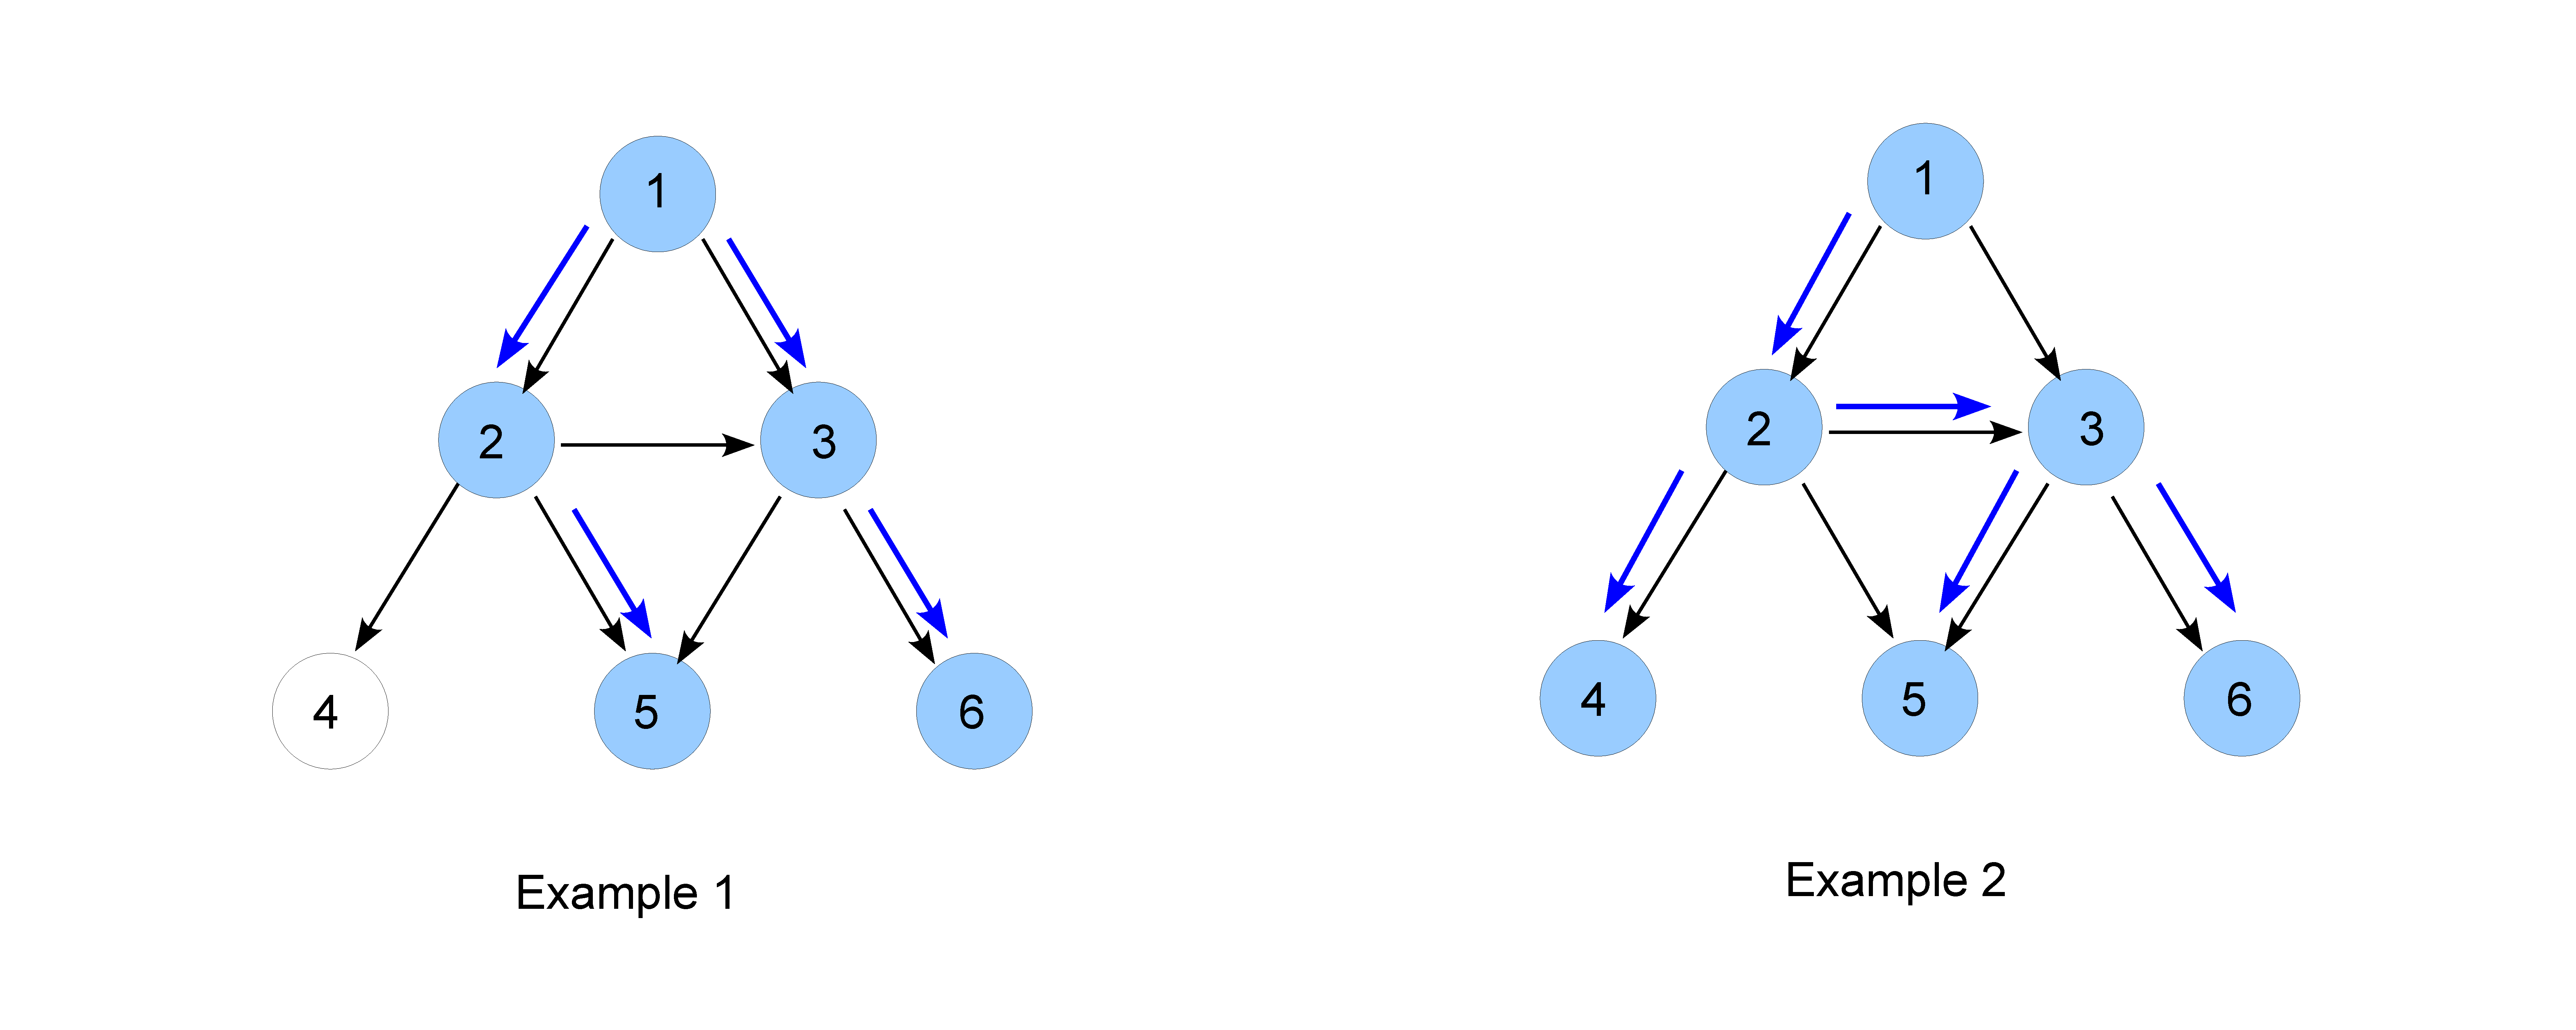
\includegraphics[width=6.5in]{flowDiagram}
\label{flowDiagram}
\caption{Examples of information flow in a 6-user network.}
\end{center}
\end{figure}

\begin{figure}[htbp]
\begin{center}
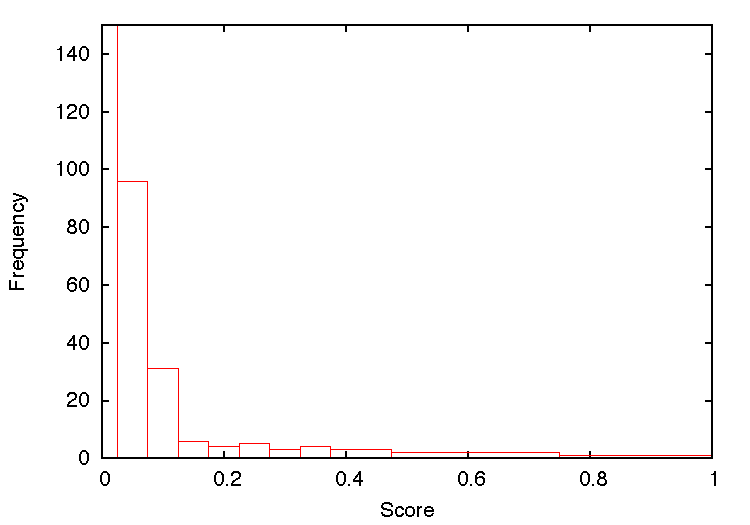
\includegraphics[width=3.5in]{L2score_15K}
\label{L2}
\caption{L2 Algorithm}
\end{center}
\end{figure}

\begin{figure}[htbp]
\begin{center}
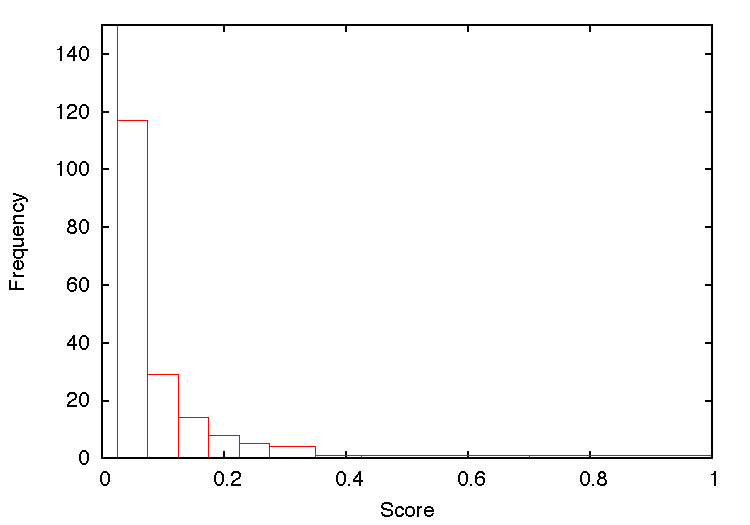
\includegraphics[width=3.5in]{L3score_15K}
\label{L3}
\caption{L3 Algorithm}
\end{center}
\end{figure}

\begin{figure}[htbp]
\begin{center}
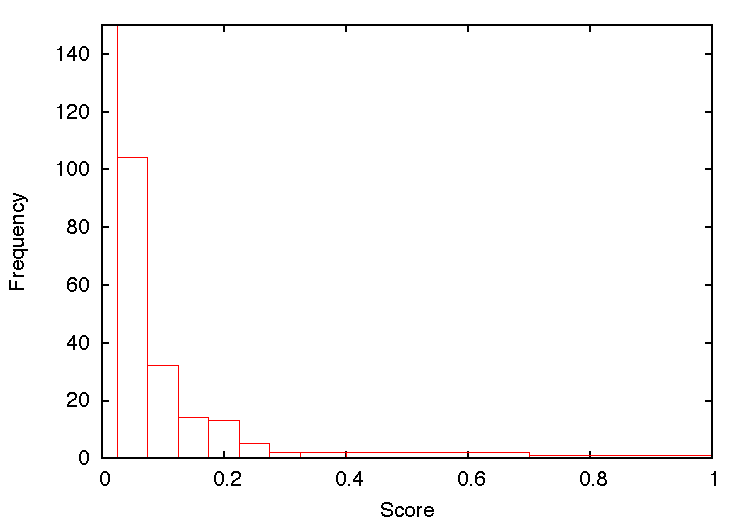
\includegraphics[width=3.5in]{L3Modscore_15K}
\label{L3Mod}
\caption{L3 Modified Algorithm}
\end{center}
\end{figure}





\subsection{Experiment 3}

In this experiment, we compare the top 150 influential users ranked by each of our algorithms.  We investigate whether or not the algorithms give similar results.  A venn diagram of the data is plotted in figure \ref{venn}.  We observe Degree count and PageRank are more similar to one another, while the L2 algorithm is somewhat different.  This is consistent with the findings of Cha et. al \cite{Cha2010}, who noted that degree count had little to do with number of mentions or retweets.




\begin{figure}[]
\begin{center}
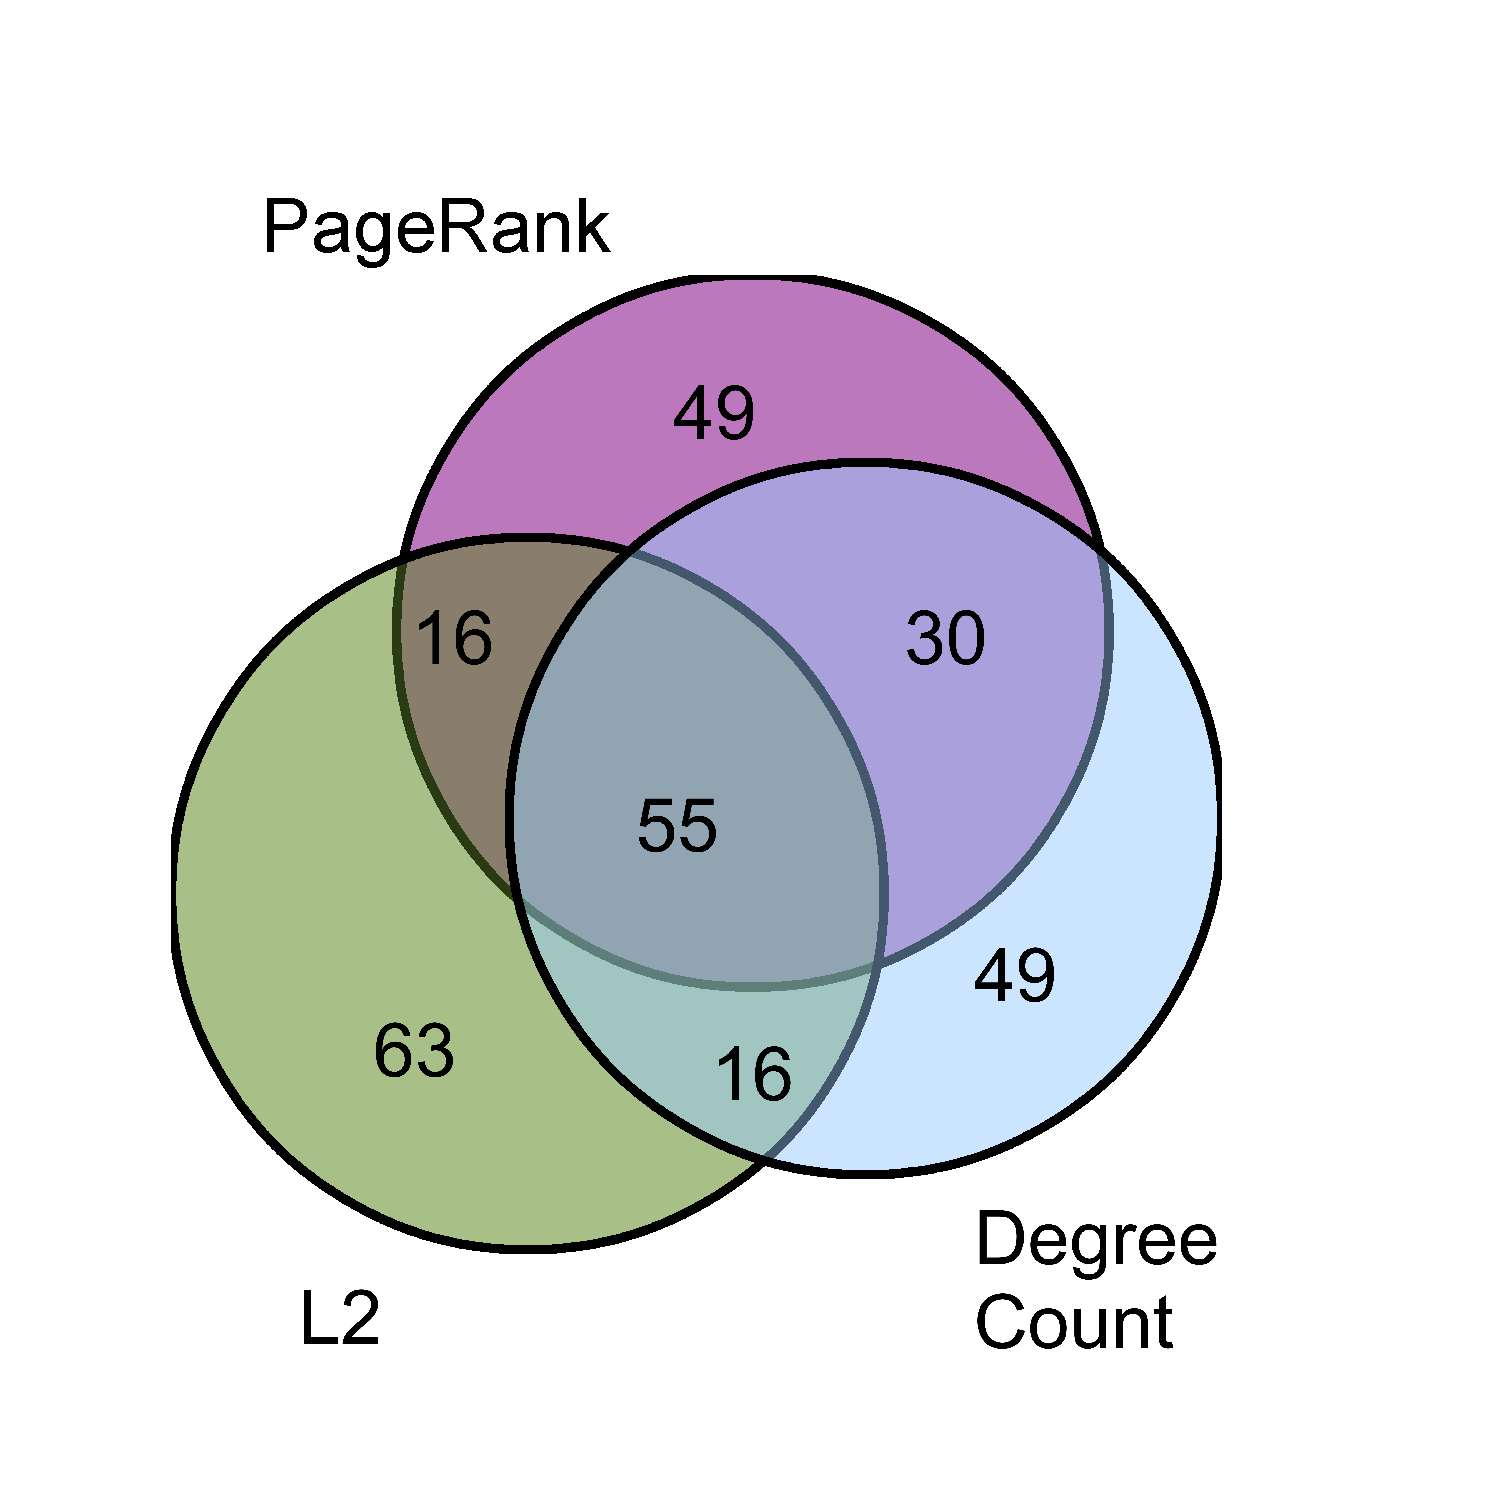
\includegraphics[width=3.5in]{venn}
\label{venn}
\caption{We examined the top 150 most influential users on the 15K dataset as ranked by our L2 algorithm, PageRank, and degree count. }
\end{center}
\end{figure}

\begin{figure}
\label{rankscomp}
\begin{tabular}{r|l|l|l}
\hline
\textbf{Rank} & \textbf{KHYRank} & \textbf{PageRank} & \textbf{Degree Count} \\
\hline
\hline
1 & \hilightr{Chris Brogan}        & Barack Obama & Barack Obama \\
2 & \hilightg{Wil Wheaton} & Twitter & Kevin Rose \\
3 & The New York Times & Kevin Rose & Zappos.com CEO -Tony \\
4 & \hilightb{Tim O'Reilly} & The Onion & Twitter  \\
5 & John Gruber & \hilightg{Wil Wheaton} & \hilightr{Chris Brogan} \\
6 & Dave Winer & Zappos.com CEO -Tony & The Onion\\
7 & The Onion & \hilightb{Tim O'Reilly} & \hilightg{Wil Wheaton} \\
8 & Wired & Leo Laporte & Jason Calacanis\\
9 & iJustine & Laughing Squid & Leo Laporte \\
10 & Felicia Day & Jason Calacanis & Chris Pirillo \\
\hline
\end{tabular}

%\begin{tabular}{|r|r|r|}
%\hline
%KHYRank & Outdegrees & PageRank\\
%\hline
%Chris Brogan & 5 & 18 \\
%Wil Wheaton & 7 & 5 \\
%The New York Times & 21 & 15 \\
%Tim O'Reilly & 13 & 7 \\
%John Gruber & 40 & 12 \\
%Dave Winer & 49 & 38 \\
%The Onion & 6 & 4 \\
%Wired & 109 & 118 \\
%iJustine & 15 & 17 \\
%Felicia Day & 18 & 11 \\
%\hline
%\end{tabular}
%%Kevin Rose & 2 & 3 \\
%%Scott Hanselman & 360 & 300 \\
%%Veronica Belmont & 12 & 14 \\
%%Reg Saddler & 16 & 49 \\
%%Dan Schawbel & 50 & 142 \\
%%
%%
%
%
%%dc & khy & pr
%%
%%
%%
%%Barack Obama & 16 & 1 \\
%%Kevin Rose & 11 & 3 \\
%%Zappos.com CEO -Tony & 31 & 6 \\
%%Twitter & 19 & 2 \\
%%Chris Brogan & 1 & 18 \\
%%The Onion & 7 & 4 \\
%%Wil Wheaton & 2 & 5 \\
%%Jason Calacanis & 2859 & 10 \\
%%Leo Laporte & 29 & 8 \\
%%Chris Pirillo & 20 & 22 \\
%%woot.com & 70 & 13 \\
%%Veronica Belmont & 13 & 14 \\
%%Tim O'Reilly & 4 & 7 \\
%%Starbucks Coffee & 18 & 20 \\
%%iJustine & 9 & 17 \\
%%
%%
%%
%%
%%pr , khy , dc
%%
%%Barack Obama & 16 & 1 \\
%%Twitter & 19 & 4 \\
%%Kevin Rose & 11 & 2 \\
%%The Onion & 7 & 6 \\
%%Wil Wheaton & 2 & 7 \\
%%Zappos.com CEO -Tony & 31 & 3 \\
%%Tim O'Reilly & 4 & 13 \\
%%Leo Laporte & 29 & 9 \\
%%Laughing Squid & 25 & 19 \\
%%Jason Calacanis & 2859 & 8 \\
%%Felicia Day & 10 & 18 \\
%%John Gruber & 5 & 40 \\
%%woot.com & 70 & 11 \\
%%Veronica Belmont & 13 & 12 \\
%%The New York Times & 3 & 21 \\
%%
%%
%%
%\-\\
%\begin{tabular}{|r|r|r|}
%\hline
%KHYRank (Layer2) & KHYRank (Layer3) & PageRank\\
%\hline
%Chris Brogan & 1 & 18 \\
%Wil Wheaton & 5 & 5 \\
%The New York Times & 3 & 15 \\
%Tim O'Reilly & 4 & 7 \\
%John Gruber & 13 & 12 \\
%Dave Winer & 2 & 38 \\
%The Onion & 15 & 4 \\
%Wired & 9 & 118 \\
%iJustine & 48 & 17 \\
%Felicia Day & 7 & 11 \\
%\hline
%\end{tabular}
%%Kevin Rose & 12 & 3 \\
%%Scott Hanselman & 16 & 300 \\
%%Veronica Belmont & 61 & 14 \\
%%Reg Saddler & 6 & 49 \\
%%Dan Schawbel & 19 & 142 \\
%%
%%
%%
%\begin{tabular}{|r|r|r|}
%\hline
%10K & 15K & 20K\\
%\hline
%Chris Brogan & 1 & 1 \\
%Wil Wheaton & 2 & 63 \\
%The New York Times & 3 & 71 \\
%Tim O'Reilly & 4 & 45 \\
%John Gruber & 7 & 60 \\
%Dave Winer & 11 & 21 \\
%The Onion & 9 & 2 \\
%Wired & 8 & 41 \\
%iJustine & 10 & 77 \\
%Felicia Day & 6 & 113 \\
%\hline
%\end{tabular}
%Kevin Rose & 5 & 51 \\
%Scott Hanselman & 15 & 31 \\
%Veronica Belmont & 12 & 116 \\
%Reg Saddler & 19 & 3 \\
%Dan Schawbel & 16 & 8 \\
\caption{Ranks Comparison}
\end{figure}

\section{Discussion}
%



As shown in figure \ref{rankscomp}, our KHYRank algorithm lists many celebrities (Tim O'Reilly, Felicia Day, Chris Brogan) and content sources (The New York Times, The Onion, Wired) as the most influential users.  By examining these users' feeds, we notice that they post frequent tweets with interesting content.
 
The histograms are unsurprising: the normalized scores show exponential decay.  However, we observe that the L3 Algorithm has a higher distribution of low scores.  The L2 and L3 Modified distributions are very similar.






\section{Related Work}

The search for influential users is a widely-studied topic.  
% TODO:
\-\\
\textbf{Twitter Network}

Cha et al. collected a twitter graph and tweet dataset, examining aspects such as in degree, retweets, and mentions. They note the difficulty in defining influence, nothing that ``there is no tangible way to measure such a force, nor is there a concrete definition of what influence means, for instance, in the spread of news''  \cite{Cha2010}. They develop several interesting conclusions.  For instance, high node degree does not necessarily correlate with influence.  Content is the main factor in determining whether a tweet gets retweeted, while a users' ``name value'' influences the number of mentions they get.  Typically, influential users focus on a specific topic, and generate intelligent, perceptive content.  

\-\\
\textbf{Defining Influential Users}

%[1] Ernesto Estrada and Desmond J. Higham. Network properties revealed through matrix functions. SIAM Rev., 52:696?714, November 2010.
% TODO Vic
%\cite{Estrada}
To find the influential users in a social network, we need to understand and quantify some underlying properties such as centrality, communicability, and betweenness measures on a general matrix, and the framework that Estrada et al. put together meets this purpose perfectly \cite{Estrada}. By using the matrix exponentials of a network's adjacency, they introduced the \emph{subgraph centrality} of node i $ \left( I+A+\frac{A^2}{2!}+\cdots+\frac{A^k}{k!}+\cdots \right)_{ii} = (exp(A))_{ii}$\cite{Estrada2} and \emph{communicability} between node i and j $(exp(A))_{ij}$ \cite{Estrada3}. Furthermore, to quantify the influence of a node,\emph{betweenness} was introduced to describe the change of communicability when the node is removed, which is defined as \[ \frac{1}{(N-1)^2-(N-1)}\sum_{i=1}^N \sum_{j=1}^N \frac{exp(A)_{ij}-exp(A-E(r))_{ij}}{exp(A)_{ij}}\]
where $i\neq j,i\neq r, j\neq r$, A-E(r) is the adjacency matrix when all edges connected to node r are removed\cite{Estrada4}.


%[2] David Kempe, Jon Kleinberg, and Eva Tardos. Maximizing the spread of in�uence through �a social network. In Proceedings of the ninth ACM SIGKDD international conference on Knowledge discovery and data mining, KDD �03, pages 137?146, New York, NY, USA, 2003. ACM.
% Vic
\-\\
\textbf{Studying the Spread of Influence}

As pointed out in a research paper by Kempe et al. at Cornell University \cite{Kempe}, selecting the most influential users in a social network is a NP-hard optimization problem, and even a provable approximation for efficient algorithms can be challenging to solve. Inspired by two diffusion models of interacting particles, \emph{Linear Threshold}\cite{Granovetter} and \emph{Independent Cascade Models}\cite{Goldenberg}, where each node can be turned on as \emph{active} from \emph{inactive} based on its neighbor weights and activating threshold, the team used a natural greedy hill-climbing approach related to \cite{Domingos} to show that the performance is guaranteed to be at least 63\% (1-1/e) of optimal, which significantly out-performs other algorithms targeting high-degree or ``central'' nodes. The group further generalized the proved strategies to more realistic marketing scenario, where marketing actions are no longer simplified as making a single node active, but rather have stochastic effects to increase a subset of nodes' probability of becoming active (and each individual has different response to each actions.) To maximize the expected size of the final active set, they applied the hill-climbing algorithm on the expected revenue with respect to a vector of investment actions.

%[3] Michael Mathioudakis, Francesco Bonchi, Carlos Castillo, Aristides Gionis, and Antti Ukkonen. Sparsi?cation of in�uence networks. In Proceedings of the 17th ACM SIGKDD international conference on Knowledge discovery and data mining, KDD �11. ACM, 2011.
%TODO Aron
%\cite{Mathioudakis}
\-\\
\textbf{The SPINE Algorithm}

When given a social graph and a list of actions propagating through it, Mathioudakis et al. designed the SPINE algorithm to find the 'backbone' of the network through the use of the independent-cascade model \cite{Mathioudakis}. The algorithm proved to be an effective pre-processing step for solving influence-maximization problems. The effectiveness of SPINE came from its ability to reduce computation speed significantly while giving up little accuracy. Its main applications included propagation characterization, feed ranking, and viral marketing.

%TODO:  Vic
 \-\\
 \textbf{PageRank}
 
Page el al. \cite{ilprints422} developed the famous PageRank algorithm behind the web search engine Google to measure and rank the importance of web contents relevant to user queries. Let $E(u)$ be a vector over a source of rank corresponding to a set of web pages. Then $R$, the PageRank, is defined as a vector satisfying \[R(u) = c\sum_{v\in B_u}\frac{R(v)}{N_v} + cE(u) = c(A + E\times \mathbf{1})R\]
Where $N_u = |F_u|$ is the count of links pointed from page $u$, $c$ is the normalizing factor such that the total rank of all pages is constant. $A_{u,v} =  1/N_u$ if $u$ links to $v$, $A_{u,v} = 0$ otherwise. The PageRank algorithm is solely based on the web linkage structure, regardless of the contents and other metadata. It emphasized on backlinks authority, meaning that more important pages have higher voting weights against the average pages. It is useful for information retrieval and finding clusterings in a web graph. 

In our experiment, we applied the PageRank algorithm in our twitter graph and compared the results with our KHYRank algorithm. We define the adjacency matrix $A$ as following: entry $A_{ij} = 1$ if user $j$ is following user $i$; otherwise, $A_{ij} = 0$. Then, we obtained the PageRank matrix $R$ through the relation\cite{arasu}
\[ \mathbf{R}(t+1) = d\mathbf{M}\mathbf{R}(t) + \frac{1-d}{N}\mathbf{1} \]
and solve for
\[ \mathbf{R} = (\mathbf{I} - d\mathbf{M})^{-1}\frac{1-d}{N}\mathbf{1}\]
where $\mathbf{M} = (K^{-1}A)^T$, $K$ is the matrix with outdegrees in diagonal and zeros in non-diagonal entries. Unsurprisingly, the results we got from this approach are very similar to the those we got from degree count, which are both solely based on the linkage structure in the network.

\-\\
\textbf{Optimization Algorithms}
%[4] Berkant Savas and Inderjit S Dhillon. Clustered low rank approximation of graphs in information science applications. In Proceedings of the 2011 SIAM International Conference on Data Mining, 2011
%TODO Vic
%\cite{Dhillon}

To approximate a massive graph of networks data, Savas and Dhillon\cite{Dhillon} provided a faster and better performance framework using clustered low rank matrices. While preserving essential information structure of a massive graph, their algorithm partitions nodes into clusters, computes low rank approximations independently, and combines each low rank approximations to obtain the approximation of the entire graph. The approximation errors were derived to have deterministic bounds using a stochastic algorithm introduced by Halko et al.\cite{Halko} The clustering approach was experimented and shown to outperform traditional approximation methods in both speed efficiency and memory usage significantly.

\-\\
\textbf{Community-based approaches}

%[5] Yu Wang, Gao Cong, Guojie Song, and Kunqing Xie. Community-based greedy algorithm for mining top-k in�uential nodes in mobile social networks. In Proceedings of the 16th ACM SIGKDD international conference on Knowledge discovery and data mining, KDD �10, pages 1039?1048, New York, NY, USA, 2010. ACM
% TODO Aron
Wang et al. took a community-based approach to finding the influential nodes by observing information diffusion \cite{Wang}. Their research targeted the mobile social network as it modeled the spread of information on a large scale. Communities within a given network were identified through a modified version of the current community detection algorithms. The changes included the addition of information diffusion as a main factor, the handling of weighted directed graphs, and the ability to modify the threshold of community decision boundaries. Instead of mining every single communities in the network, they allowed the mining decision to be dynamically chosen by the algorithm. The selection of algorithm for finding top-K influential user is trivial. This new algorithm provided provable performance guarantee just like previous algorithms. When tested on a network with 15 times more user nodes than previous testing, the new algorithm proved to be orders of magnitude faster than the leading greedy algorithm, while maintaining a small error margin.


%[6] Andrea Galeotti, Sanjeev Goyal, Matthew O. Jackson, Fernando Vega-Redondo, and Leeat Yariv. Network games. Review of Economic Studies, 77, 2010.
% TODO Ann
\-\\
\textbf{Game Model}

The dynamics of friendship and information sharing in a social network fit into Galeotti et al.'s model of Network Games \cite{Galeotti}.  Here, players are connected in a graph.  Players can either act or not act. In a game of \emph{strategic substitutes}, a neighbor's action replaces the need for the player to act.  In the \emph{strategic complements} game, a neighbor's action gives the player greater incentive to act, while a neighbor's inaction gives the player less incentive to act.  Viral marking in a social network displays features of both strategic complements and substitutes.  For instance, if Alice shares content, her friend Bob may feel less need to duplicate content, since typically some of their friends (including Charlie) overlap.  Perhaps Charlie only needs to hear the campaign once to be influenced.  However, we might also imagine that Charlie would be more interested in the campaign if many of his friends were sharing information about it.




% Write updates for newer papers


%TODO (Ann)
\-\\
\textbf{Using topic information to determine influence}

A study by Weng et al. discovers high reciprocity for following in Twitter.  They also extend the PageRank algorithm into TwitterRank, an algorithm for finding influence.  Unlike other approaches, TwitterRank considers the topics on which users tweet when determining influence.  The authors observe that twitter users often follow others because of a shared topic of interest.  They also argue that degree count is a weak indicator of influence. They demonstrate that their algorithm outperforms follower count and traditional PageRank \cite{Weng:2010}.

\-\\
\textbf{Order of information adoption}

Lee et al. also build on the PageRank algorithm, adding a component that considers the order of information adoption in Twitter.  They study information diffusion on a real dataset, and learn that topics have a short lifespan.  Topics initially spread quickly, then die down in popularity.  They conclude that ``early tweets spread better'' \cite{Lee:2010}.
%

\-\\
\textbf{Modeling message flow}

Ye and Wu modeled message flow using a tree structure.  They also examine content with multiple sources, as well as study a dataset of 500K messages relating to Michael Jackson's death, which is famous for breaking on Twitter before traditional news outlets.  They learn that most replies happen soon after the original message.  Furthermore, they observe that messages can propagate far through the graph.  \cite{Ye:2010}
%
%\cite{Abel11}


\section{Conclusion}
%TODO

We have built our own algorithm for predicting influence on Twitter, using real data from mentions and retweets.   We compared it to traditional influence algorithms such as PageRank and degree count, and find that our algorithm does well at finding celebrities and content sources.



Please see \url{http://khyrank.cvhu.org} for implementation details.

\section{Acknowledgements}
%TODO: Would you like to thank anyone?  Your mom, cat, a friend?  Thank God the class is over?  ;)
We would like to thank Joe Reisinger for providing a dataset for our preliminary work.  We would also like to thank Charlie Schmidt and his belated cat Fatso.  You are a source of inspiration.



\bibliography{FinalWriteup}{}
\bibliographystyle{plain}

\end{document}  